\documentclass{beamer}
\usepackage[utf8]{inputenc}
\usepackage[english]{babel}
\usepackage[T1]{fontenc}
\usepackage{slide_helper}
\usepackage[inline]{asymptote}
\usepackage{asy_helper}
\usepackage[super]{nth}
\usepackage{array}
\usepackage{wasysym}
\usepackage{pgfplots}
\pgfplotsset{compat=1.5} 
\usepgfplotslibrary{statistics}

\DeclareSymbolFont{extraup}{U}{zavm}{m}{n}
\DeclareMathSymbol{\varheart}{\mathalpha}{extraup}{86}
\DeclareMathSymbol{\vardiamond}{\mathalpha}{extraup}{87}
\DeclareMathSymbol{\varclub}{\mathalpha}{extraup}{84} 
\DeclareMathSymbol{\varspade}{\mathalpha}{extraup}{85}

\newcommand{\suitheart}[1][]{{\color{red}\text{#1}\varheart}}
\newcommand{\suitspade}[1][]{{\color{black}\text{#1}\spadesuit}}
\newcommand{\suitdiamond}[1][]{{\color{red}\text{#1}\vardiamond}}
\newcommand{\suitclub}[1][]{{\color{black}\text{#1}\varclub}}

\newcommand{\prob}[1]{P\left(#1\right)}
\newcommand{\condprob}[2]{\prob{#1~\middle|~#2}}
\newcommand{\comb}[2]{{_{#1}C_{#2}}}
\newcommand{\perm}[2]{_{#1}P_{#2}}

\newcommand{\nullhypothesis}[1]{H_0&:~{#1}}
\newcommand{\althypothesis}[1]{H_A&:~{#1}}

\begin{asydef}
real nd_func(real mu, real sigma, real x) { return 1/sqrt(2*pi*sigma*sigma)*exp((-1*(x-mu)*(x-mu))/(2*sigma*sigma)); }

guide normal_dist(real mu, real sigma, real xmin, real xmax)
{
	real f(real x) { return nd_func(mu, sigma, x); }
	return graph(f, xmin, xmax);
}

void shade_between(real mu, real sigma, real a, real b, pen p=orange)
{
	real f(real x) { return nd_func(mu, sigma, x); }
	guide g = graph(f, a, b);
	
	filldraw((a,0) -- g -- (b,0) -- cycle, p, black);
}

void multiple_nd_curves_example(real std_dev)
{
	size(300, 190, IgnoreAspect);
    
    draw(normal_dist(0, std_dev, -6,6));
    shade_between(0,std_dev,-std_dev,std_dev);
    draw((0,0)--(0,0.45));
    
    label("$\sigma="+format("%#.2f", std_dev)+"$", (-4.2,0.45), Fill(paleyellow));
    
    xaxis(Bottom(), RightTicks(new real[] {-6,-4,-2,0,2,4,6}));
    yaxis(Left(), LeftTicks(size=nan),ymin = 0, ymax = 0.5);
}
\end{asydef}

\begin{asydef}
pair crit = (150, 33);
real a=-1.25;
real b=1.25;
\end{asydef}

\title[MA205 - Section 10.1]{Correlation}

\begin{document}
\begin{frame}
\titlepage
\end{frame}

\begin{frame}\small
\begin{definition}
A \textbf{correlation} exists between two variables when the values of one variable are somehow associated with the values of the other variables.
\end{definition}\pause

\begin{definition}
A \textbf{linear correlation} exists between two variables when there is a correlation and the plotted points of paired data result in a pattern that can be approximated by a straight line.
\end{definition}\pause

\begin{definition}
A \textbf{scatterplot} is a plot of paired $(x,y)$ quantitative data with a horizontal x-axis and a vertical y-axis. The horizontal axis is used for the first variable ($x$), and the vertical axis for the second variable ($y$).
\end{definition}\pause

\begin{note}
Because conclusions based on visual examinations of scatterplots are largely subjective, we need more objective measures. We use the linear correlation coefficient $r$, which is a number that measures the strength of the linear association between the two variables.
\end{note}
\end{frame}

\begin{frame}
\begin{example}
\begin{center}
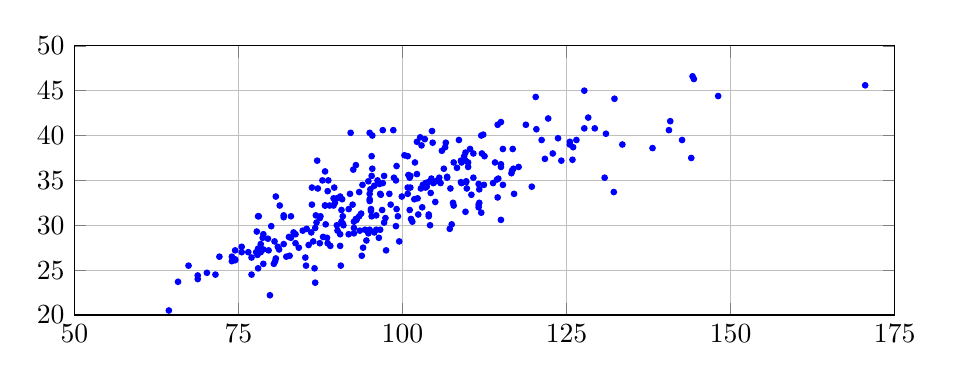
\begin{tikzpicture}
\pgfkeys{/pgf/number format/.cd,
fixed,
precision=999,
set thousands separator={},
1000 sep in fractionals=false,
}
\begin{axis}[
width=12cm,
height=5.0cm,
%xlabel={Waist Circumference (cm)},
%ylabel={Arm Circumference (cm)},
ymajorgrids=true,
xmajorgrids=true,
%enlarge x limits=false,
%enlarge y limits=false,
xticklabel style={/pgf/number format/.cd,fixed,precision=0},
xticklabel=\pgfmathprintnumber{\tick},
xtick={50,75,...,175},
ytick={20,25,...,50},
ymin=20,
ymax=50,
xmin=50,
xmax=175,
scatter/use mapped color={
 %draw=mapped color,
 fill=blue,
},
]
\addplot[scatter, only marks, blue, scatter src=y, mark size=1pt]
coordinates
{
(	120.4	,	40.7	)
(	107.8	,	37	)
(	120.3	,	44.3	)
(	97.2	,	30.3	)
(	95.1	,	34	)
(	112	,	31.4	)
(	78	,	27.4	)
(	103.5	,	34.2	)
(	89.7	,	32.5	)
(	112	,	40	)
(	95	,	32.7	)
(	115.3	,	38.5	)
(	118.8	,	41.2	)
(	92.6	,	30.4	)
(	75.5	,	27	)
(	101.8	,	32.9	)
(	92.5	,	36.2	)
(	100.8	,	33.5	)
(	82.8	,	26.6	)
(	92.9	,	36.7	)
(	109	,	34.7	)
(	101.9	,	37	)
(	110	,	36.5	)
(	102.3	,	33	)
(	80	,	29.9	)
(	94.3	,	29.5	)
(	103.1	,	34.5	)
(	103	,	32	)
(	90.5	,	29	)
(	88.2	,	36	)
(	78.8	,	29	)
(	65.8	,	23.7	)
(	114.4	,	35.1	)
(	78	,	25.2	)
(	106.8	,	35.4	)
(	112.4	,	34.5	)
(	94.8	,	34.9	)
(	90.6	,	25.5	)
(	95.2	,	31.8	)
(	71.5	,	24.5	)
(	94.5	,	28.3	)
(	95.3	,	31	)
(	103.5	,	34.7	)
(	104.2	,	30	)
(	88.7	,	35	)
(	109.7	,	34.9	)
(	115	,	36.8	)
(	64.4	,	20.5	)
(	133.5	,	39	)
(	102.2	,	39.3	)
(	138.1	,	38.6	)
(	112.1	,	38	)
(	70.2	,	24.7	)
(	144.4	,	46.3	)
(	95.7	,	29.2	)
(	98.7	,	35.3	)
(	121.7	,	37.4	)
(	87.4	,	28	)
(	77.7	,	27	)
(	100.9	,	35.6	)
(	93.4	,	33.7	)
(	125.9	,	37.3	)
(	121.2	,	39.5	)
(	90.5	,	27.7	)
(	86.7	,	23.6	)
(	82.3	,	26.5	)
(	107.3	,	34.1	)
(	88.2	,	32.2	)
(	129.3	,	40.8	)
(	78.8	,	25.7	)
(	95	,	29.5	)
(	102.8	,	34.1	)
(	85.3	,	25.5	)
(	79.6	,	27.2	)
(	101.2	,	34.2	)
(	111.6	,	32	)
(	90.8	,	32.9	)
(	108.6	,	39.5	)
(	81.9	,	30.9	)
(	132.2	,	33.7	)
(	87	,	37.2	)
(	108.9	,	37.2	)
(	74.5	,	27.2	)
(	107.7	,	32.5	)
(	96	,	29.5	)
(	79.5	,	28.5	)
(	111.7	,	34	)
(	83	,	28.6	)
(	80.6	,	26	)
(	102.4	,	31.2	)
(	96.7	,	33.4	)
(	93	,	30.6	)
(	88.6	,	28	)
(	97	,	40.6	)
(	95.4	,	36.3	)
(	104.5	,	40.5	)
(	106.3	,	36.3	)
(	97.2	,	35.5	)
(	140.8	,	41.6	)
(	90.5	,	33.2	)
(	98.6	,	40.6	)
(	115	,	41.5	)
(	98.2	,	32.3	)
(	114.5	,	33.1	)
(	108.9	,	34.8	)
(	80.7	,	26.3	)
(	96.9	,	31.7	)
(	95.4	,	40	)
(	100.8	,	37.7	)
(	99.1	,	36.6	)
(	88.6	,	33.8	)
(	87.8	,	35	)
(	105.6	,	35.3	)
(	103.4	,	39.6	)
(	116.6	,	35.8	)
(	85.7	,	27.8	)
(	90.9	,	30.2	)
(	89.5	,	33	)
(	89	,	27.7	)
(	77.8	,	29.3	)
(	77.9	,	26.7	)
(	104	,	31.2	)
(	105.1	,	34.9	)
(	84.8	,	29.4	)
(	127.7	,	40.8	)
(	81.9	,	31.1	)
(	126.5	,	39.5	)
(	83	,	31	)
(	96.4	,	28.6	)
(	106	,	38.3	)
(	83.7	,	29	)
(	101.2	,	35.5	)
(	96.2	,	35	)
(	104.6	,	39.2	)
(	77	,	24.5	)
(	115	,	30.6	)
(	86.1	,	29.2	)
(	102.2	,	35.7	)
(	93.9	,	34.5	)
(	92.4	,	32.3	)
(	110.3	,	38.5	)
(	127.7	,	45	)
(	99.1	,	31.8	)
(	109.8	,	34.1	)
(	95.2	,	31.6	)
(	99	,	29.9	)
(	87.9	,	28.7	)
(	123.7	,	39.7	)
(	107.2	,	29.6	)
(	86.4	,	28.2	)
(	90.7	,	30.4	)
(	68.8	,	24.4	)
(	68.8	,	24	)
(	99.3	,	31	)
(	140.6	,	40.6	)
(	119.7	,	34.3	)
(	83.7	,	28	)
(	96.6	,	33.5	)
(	99	,	35	)
(	88.2	,	32.2	)
(	87.5	,	31	)
(	81.9	,	27.9	)
(	97.5	,	27.2	)
(	106.6	,	39.2	)
(	91	,	30	)
(	80.4	,	25.7	)
(	107.8	,	32.2	)
(	76.5	,	27	)
(	115.3	,	34.5	)
(	95.3	,	35.5	)
(	109.6	,	38.1	)
(	110.8	,	38	)
(	92.9	,	30.7	)
(	114.5	,	41.2	)
(	109.6	,	37.2	)
(	122.9	,	38	)
(	78.8	,	27.3	)
(	92	,	33.5	)
(	99.5	,	28.2	)
(	114.6	,	35.2	)
(	90	,	30	)
(	87.1	,	34.1	)
(	93.5	,	29.4	)
(	170.5	,	45.6	)
(	105.8	,	34.7	)
(	100.3	,	37.8	)
(	92.6	,	29.7	)
(	88.3	,	30.1	)
(	110.5	,	33.4	)
(	102.7	,	39.8	)
(	112.5	,	37.7	)
(	105.4	,	35	)
(	132.3	,	44.1	)
(	104.3	,	33.6	)
(	94.8	,	29.1	)
(	85.4	,	29.6	)
(	96.5	,	34.6	)
(	109.6	,	31.5	)
(	106.5	,	38.7	)
(	79.8	,	22.2	)
(	84.2	,	27.5	)
(	89.5	,	32.2	)
(	90.1	,	29.4	)
(	116.8	,	38.5	)
(	148.1	,	44.4	)
(	93.4	,	31	)
(	77	,	26.4	)
(	116.7	,	36.1	)
(	101.5	,	30.4	)
(	112.3	,	40.1	)
(	96.6	,	29.5	)
(	83.4	,	29.2	)
(	81.3	,	32.2	)
(	144.2	,	46.6	)
(	103.7	,	34.3	)
(	95.7	,	34.4	)
(	81	,	27.6	)
(	126	,	38.7	)
(	89.6	,	34.2	)
(	98	,	33.5	)
(	110.8	,	35.3	)
(	104	,	31	)
(	99.9	,	33.2	)
(	95.3	,	37.7	)
(	105	,	32.6	)
(	131	,	40.2	)
(	125.5	,	39.3	)
(	80.7	,	33.2	)
(	110	,	37	)
(	130.8	,	35.3	)
(	78.7	,	28.6	)
(	97	,	34.7	)
(	88.9	,	32.2	)
(	90.7	,	31.7	)
(	86.9	,	30.3	)
(	95	,	32.9	)
(	80.5	,	28.2	)
(	104.4	,	35.2	)
(	74	,	26	)
(	104.7	,	34.7	)
(	101.3	,	30.7	)
(	82.7	,	28.7	)
(	115	,	36.5	)
(	72.1	,	26.5	)
(	95	,	40.3	)
(	96	,	31.1	)
(	87.4	,	30.8	)
(	111.7	,	32.5	)
(	111.6	,	32.3	)
(	74.5	,	26.2	)
(	128.3	,	42	)
(	102.9	,	38.9	)
(	108.3	,	36.4	)
(	94	,	27.5	)
(	81.2	,	27.3	)
(	122.2	,	41.9	)
(	75.5	,	27.6	)
(	109.4	,	37.7	)
(	91.8	,	29	)
(	114.1	,	37	)
(	124.2	,	37.2	)
(	111.6	,	34.6	)
(	116.9	,	36.3	)
(	86.8	,	31.1	)
(	86.6	,	25.2	)
(	86.2	,	32.3	)
(	92.6	,	29.1	)
(	109.7	,	34.8	)
(	106.8	,	35.3	)
(	93.8	,	26.6	)
(	100.8	,	34.2	)
(	117	,	33.5	)
(	78.4	,	27	)
(	86.7	,	29.7	)
(	91.8	,	31.8	)
(	85.2	,	26.4	)
(	93.7	,	31.3	)
(	144	,	37.5	)
(	113.8	,	34.7	)
(	103.9	,	34.8	)
(	95	,	33.5	)
(	78	,	31	)
(	101.1	,	35.3	)
(	107.5	,	30.1	)
(	97.4	,	30.8	)
(	90.9	,	31	)
(	88.5	,	28.6	)
(	67.4	,	25.5	)
(	92.1	,	40.3	)
(	101.1	,	31.7	)
(	78.1	,	31	)
(	90	,	33	)
(	125.5	,	39	)
(	86.2	,	34.2	)
(	74.5	,	26.1	)
(	78.4	,	27.9	)
(	142.6	,	39.5	)
(	117.7	,	36.5	)
(	109	,	37	)
(	74	,	26.5	)
};
\end{axis}
\end{tikzpicture}
\end{center}\pause
Distinct straight-line, or linear, pattern. We say that there is a positive linear correlation ($r=0.80241$) between $x$ and $y$, since as the $x$ values increase, the corresponding $y$ values also increase.
\end{example}
\end{frame}

\begin{frame}
\begin{example}
\begin{center}
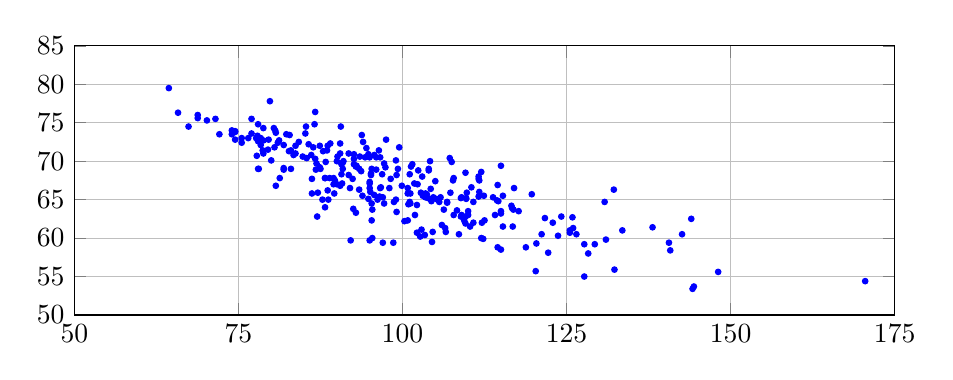
\begin{tikzpicture}
\pgfkeys{/pgf/number format/.cd,
fixed,
precision=999,
set thousands separator={},
1000 sep in fractionals=false,
}
\begin{axis}[
width=12cm,
height=5.0cm,
%xlabel={Waist Circumference (cm)},
%ylabel={Arm Circumference (cm)},
ymajorgrids=true,
xmajorgrids=true,
%enlarge x limits=false,
%enlarge y limits=false,
xticklabel style={/pgf/number format/.cd,fixed,precision=0},
xticklabel=\pgfmathprintnumber{\tick},
xtick={50,75,...,175},
ytick={50,55,...,100},
ymin=50,
ymax=85,
xmin=50,
xmax=175,
scatter/use mapped color={
 %draw=mapped color,
 fill=blue,
},
]
\addplot[scatter, only marks, blue, scatter src=y, mark size=1pt]
coordinates
{
(120.4,59.3)
(107.8,63)
(120.3,55.7)
(97.2,69.7)
(95.1,66)
(112,68.6)
(78,72.6)
(103.5,65.8)
(89.7,67.5)
(112,60)
(95,67.3)
(115.3,61.5)
(118.8,58.8)
(92.6,69.6)
(75.5,73)
(101.8,67.1)
(92.5,63.8)
(100.8,66.5)
(82.8,73.4)
(92.9,63.3)
(109,65.3)
(101.9,63)
(110,63.5)
(102.3,67)
(80,70.1)
(94.3,70.5)
(103.1,65.5)
(103,68)
(90.5,71)
(88.2,64)
(78.8,71)
(65.8,76.3)
(114.4,64.9)
(78,74.8)
(106.8,64.6)
(112.4,65.5)
(94.8,65.1)
(90.6,74.5)
(95.2,68.2)
(71.5,75.5)
(94.5,71.7)
(95.3,69)
(103.5,65.3)
(104.2,70)
(88.7,65)
(109.7,65.1)
(115,63.2)
(64.4,79.5)
(133.5,61)
(102.2,60.7)
(138.1,61.4)
(112.1,62)
(70.2,75.3)
(144.4,53.7)
(95.7,70.8)
(98.7,64.7)
(121.7,62.6)
(87.4,72)
(77.7,73)
(100.9,64.4)
(93.4,66.3)
(125.9,62.7)
(121.2,60.5)
(90.5,72.3)
(86.7,76.4)
(82.3,73.5)
(107.3,65.9)
(88.2,67.8)
(129.3,59.2)
(78.8,74.3)
(95,70.5)
(102.8,65.9)
(85.3,74.5)
(79.6,72.8)
(101.2,65.8)
(111.6,68)
(90.8,67.1)
(108.6,60.5)
(81.9,69.1)
(132.2,66.3)
(87,62.8)
(108.9,62.8)
(74.5,72.8)
(107.7,67.5)
(96,70.5)
(79.5,71.5)
(111.7,66)
(83,71.4)
(80.6,74)
(102.4,68.8)
(96.7,66.6)
(93,69.4)
(88.6,72)
(97,59.4)
(95.4,63.7)
(104.5,59.5)
(106.3,63.7)
(97.2,64.5)
(140.8,58.4)
(90.5,66.8)
(98.6,59.4)
(115,58.5)
(98.2,67.7)
(114.5,66.9)
(108.9,65.2)
(80.7,73.7)
(96.9,68.3)
(95.4,60)
(100.8,62.3)
(99.1,63.4)
(88.6,66.2)
(87.8,65)
(105.6,64.7)
(103.4,60.4)
(116.6,64.2)
(85.7,72.2)
(90.9,69.8)
(89.5,67)
(89,72.3)
(77.8,70.7)
(77.9,73.3)
(104,68.8)
(105.1,65.1)
(84.8,70.6)
(127.7,59.2)
(81.9,68.9)
(126.5,60.5)
(83,69)
(96.4,71.4)
(106,61.7)
(83.7,71)
(101.2,64.5)
(96.2,65)
(104.6,60.8)
(77,75.5)
(115,69.4)
(86.1,70.8)
(102.2,64.3)
(93.9,65.5)
(92.4,67.7)
(110.3,61.5)
(127.7,55)
(99.1,68.2)
(109.8,65.9)
(95.2,68.4)
(99,70.1)
(87.9,71.3)
(123.7,60.3)
(107.2,70.4)
(86.4,71.8)
(90.7,69.6)
(68.8,75.6)
(68.8,76)
(99.3,69)
(140.6,59.4)
(119.7,65.7)
(83.7,72)
(96.6,66.5)
(99,65)
(88.2,67.8)
(87.5,69)
(81.9,72.1)
(97.5,72.8)
(106.6,60.8)
(91,70)
(80.4,74.3)
(107.8,67.8)
(76.5,73)
(115.3,65.5)
(95.3,64.5)
(109.6,61.9)
(110.8,62)
(92.9,69.3)
(114.5,58.8)
(109.6,62.8)
(122.9,62)
(78.8,72.7)
(92,66.5)
(99.5,71.8)
(114.6,64.8)
(90,70)
(87.1,65.9)
(93.5,70.6)
(170.5,54.4)
(105.8,65.3)
(100.3,62.2)
(92.6,70.3)
(88.3,69.9)
(110.5,66.6)
(102.7,60.2)
(112.5,62.3)
(105.4,65)
(132.3,55.9)
(104.3,66.4)
(94.8,70.9)
(85.4,70.4)
(96.5,65.4)
(109.6,68.5)
(106.5,61.3)
(79.8,77.8)
(84.2,72.5)
(89.5,67.8)
(90.1,70.6)
(116.8,61.5)
(148.1,55.6)
(93.4,69)
(77,73.6)
(116.7,63.9)
(101.5,69.6)
(112.3,59.9)
(96.6,70.5)
(83.4,70.8)
(81.3,67.8)
(144.2,53.4)
(103.7,65.7)
(95.7,65.6)
(81,72.4)
(126,61.3)
(89.6,65.8)
(98,66.5)
(110.8,64.7)
(104,69)
(99.9,66.8)
(95.3,62.3)
(105,67.4)
(131,59.8)
(125.5,60.7)
(80.7,66.8)
(110,63)
(130.8,64.7)
(78.7,71.4)
(97,65.3)
(88.9,67.8)
(90.7,68.3)
(86.9,69.7)
(95,67.1)
(80.5,71.8)
(104.4,64.8)
(74,74)
(104.7,65.3)
(101.3,69.3)
(82.7,71.3)
(115,63.5)
(72.1,73.5)
(95,59.7)
(96,68.9)
(87.4,69.2)
(111.7,67.5)
(111.6,67.7)
(74.5,73.8)
(128.3,58)
(102.9,61.1)
(108.3,63.6)
(94,72.5)
(81.2,72.7)
(122.2,58.1)
(75.5,72.4)
(109.4,62.3)
(91.8,71)
(114.1,63)
(124.2,62.8)
(111.6,65.4)
(116.9,63.7)
(86.8,68.9)
(86.6,74.8)
(86.2,67.7)
(92.6,70.9)
(109.7,65.2)
(106.8,64.7)
(93.8,73.4)
(100.8,65.8)
(117,66.5)
(78.4,73)
(86.7,70.3)
(91.8,68.2)
(85.2,73.6)
(93.7,68.7)
(144,62.5)
(113.8,65.3)
(103.9,65.2)
(95,66.5)
(78,69)
(101.1,64.7)
(107.5,69.9)
(97.4,69.2)
(90.9,69)
(88.5,71.4)
(67.4,74.5)
(92.1,59.7)
(101.1,68.3)
(78.1,69)
(90,67)
(125.5,61)
(86.2,65.8)
(74.5,73.9)
(78.4,72.1)
(142.6,60.5)
(117.7,63.5)
(109,63)
(74,73.5)
};
\end{axis}
\end{tikzpicture}
\end{center}\pause
Distinct straight-line, or linear, pattern. We say that there is a positive linear correlation ($r=-0.80241$) between $x$ and $y$, since as the $x$ values increase, the corresponding $y$ values also increase.
\end{example}
\end{frame}

\begin{frame}%0.08161
\begin{example}
\begin{center}
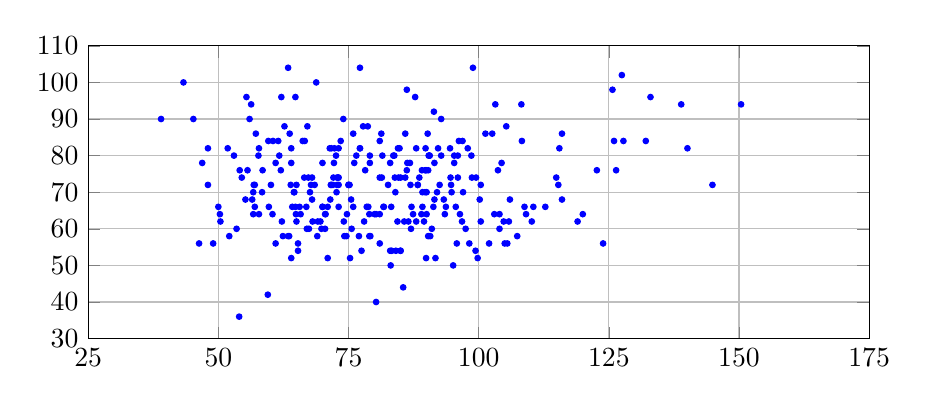
\begin{tikzpicture}
\pgfkeys{/pgf/number format/.cd,
fixed,
precision=999,
set thousands separator={},
1000 sep in fractionals=false,
}
\begin{axis}[
width=11.5cm,
height=5.3cm,
%xlabel={Weight (kg)},
%ylabel={Pulse Rate (bpm)},
ymajorgrids=true,
xmajorgrids=true,
%enlarge x limits=false,
%enlarge y limits=false,
xticklabel style={/pgf/number format/.cd,fixed,precision=0},
xticklabel=\pgfmathprintnumber{\tick},
xtick={25,50,...,175},
ytick={30,40,...,110},
ymin=30,
ymax=110,
xmin=25,
xmax=175,
scatter/use mapped color={
 %draw=mapped color,
 fill=blue,
},
]
\addplot[scatter, only marks, blue, scatter src=y, mark size=1pt]
coordinates
{
(	98.6	,	80.0	)
(	96.9	,	84	)
(	108.2	,	94.0	)
(	73.1	,	74.0	)
(	83.1	,	50	)
(	87	,	60.0	)
(	64	,	52.0	)
(	79.2	,	58.0	)
(	64.2	,	66.0	)
(	119	,	62	)
(	71	,	52.0	)
(	98.2	,	56.0	)
(	122.7	,	76.0	)
(	75.3	,	52.0	)
(	51.8	,	82	)
(	76.1	,	78.0	)
(	89.5	,	62.0	)
(	75.9	,	86.0	)
(	67.1	,	88.0	)
(	86.9	,	72.0	)
(	91	,	60.0	)
(	96.4	,	64	)
(	81	,	56.0	)
(	86.3	,	78	)
(	54	,	36.0	)
(	72.3	,	82.0	)
(	78.5	,	66.0	)
(	71	,	66	)
(	60.5	,	84	)
(	75.9	,	66	)
(	55.6	,	76	)
(	46.9	,	78.0	)
(	93.5	,	64.0	)
(	50	,	66.0	)
(	86.8	,	78.0	)
(	87.8	,	96.0	)
(	69.8	,	60.0	)
(	57.8	,	64.0	)
(	73.5	,	84.0	)
(	57.8	,	82.0	)
(	59.5	,	42.0	)
(	81.3	,	86	)
(	88.3	,	72.0	)
(	72.7	,	70	)
(	66.5	,	74	)
(	85.9	,	86.0	)
(	103	,	64.0	)
(	39.0	,	90.0	)
(	105.3	,	88	)
(	94.7	,	72.0	)
(	144.9	,	72.0	)
(	92.8	,	90	)
(	45.2	,	90.0	)
(	150.4	,	94.0	)
(	71.5	,	68.0	)
(	84.1	,	54.0	)
(	112.8	,	66.0	)
(	74.0	,	90	)
(	64.0	,	82	)
(	92.8	,	80.0	)
(	85.9	,	74.0	)
(	105.5	,	56.0	)
(	123.9	,	56.0	)
(	76.5	,	80.0	)
(	43.3	,	100.0	)
(	71.7	,	72.0	)
(	90.0	,	64.0	)
(	70.6	,	64.0	)
(	114.9	,	74.0	)
(	64.8	,	96.0	)
(	77	,	58.0	)
(	89.1	,	76.0	)
(	58.5	,	76.0	)
(	57.2	,	86.0	)
(	93.7	,	66.0	)
(	81.4	,	74	)
(	95.6	,	66.0	)
(	107.4	,	58.0	)
(	74.6	,	58.0	)
(	106.0	,	68.0	)
(	84	,	70.0	)
(	86.5	,	62.0	)
(	59.6	,	84.0	)
(	79.1	,	78.0	)
(	68	,	68.0	)
(	63.4	,	58.0	)
(	85.7	,	62	)
(	70	,	78.0	)
(	50.4	,	62	)
(	72.1	,	74.0	)
(	77.2	,	104.0	)
(	70	,	66.0	)
(	63.7	,	86	)
(	90	,	70.0	)
(	83.3	,	54.0	)
(	88.6	,	74.0	)
(	99.4	,	54.0	)
(	84.6	,	74.0	)
(	127.8	,	84.0	)
(	88.3	,	72.0	)
(	94.6	,	74.0	)
(	120	,	64.0	)
(	78.8	,	66.0	)
(	81.0	,	84.0	)
(	84.4	,	62.0	)
(	53.5	,	60.0	)
(	74.1	,	62.0	)
(	91.7	,	52	)
(	89.8	,	82.0	)
(	77.5	,	54.0	)
(	66.2	,	84.0	)
(	69.1	,	62	)
(	83.0	,	54.0	)
(	98.9	,	104.0	)
(	91.5	,	78.0	)
(	59.7	,	66.0	)
(	65.3	,	56.0	)
(	78.7	,	88	)
(	57	,	66.0	)
(	61.5	,	84.0	)
(	65.8	,	64.0	)
(	80	,	64.0	)
(	83.0	,	78.0	)
(	63.4	,	104.0	)
(	126.4	,	76.0	)
(	66.6	,	84.0	)
(	126.0	,	84.0	)
(	65	,	62	)
(	71.7	,	82.0	)
(	104	,	64.0	)
(	64.0	,	78	)
(	94.8	,	70.0	)
(	78.2	,	76	)
(	90.2	,	86.0	)
(	48	,	72.0	)
(	88	,	82.0	)
(	64.8	,	66.0	)
(	95.1	,	50.0	)
(	77.2	,	82.0	)
(	80.3	,	40.0	)
(	99.5	,	74.0	)
(	110.5	,	66	)
(	83.9	,	74.0	)
(	86.2	,	76.0	)
(	81.8	,	66.0	)
(	70	,	66.0	)
(	62.4	,	58.0	)
(	105.8	,	62.0	)
(	83.8	,	80.0	)
(	63.6	,	58.0	)
(	77.2	,	82.0	)
(	50.3	,	64.0	)
(	48.0	,	82	)
(	89.7	,	76	)
(	132.1	,	84.0	)
(	92.0	,	70.0	)
(	62.7	,	88	)
(	85.5	,	44.0	)
(	81	,	64	)
(	81.5	,	80.0	)
(	68.1	,	62	)
(	56.7	,	70.0	)
(	73.1	,	82.0	)
(	95.3	,	78.0	)
(	68	,	74	)
(	52.1	,	58.0	)
(	87.4	,	64.0	)
(	55.2	,	68	)
(	89.7	,	70.0	)
(	80.3	,	64.0	)
(	90.3	,	58.0	)
(	89.9	,	52	)
(	67.0	,	60.0	)
(	100.4	,	72.0	)
(	95.3	,	80.0	)
(	97.0	,	70	)
(	54.5	,	74.0	)
(	75	,	72.0	)
(	65.6	,	66.0	)
(	108.8	,	66.0	)
(	69	,	58	)
(	73.0	,	74.0	)
(	67.6	,	70.0	)
(	140.1	,	82.0	)
(	91.3	,	66.0	)
(	86.2	,	98.0	)
(	72.8	,	74.0	)
(	73.1	,	72.0	)
(	81.7	,	66.0	)
(	99.8	,	52.0	)
(	97.9	,	82.0	)
(	90.4	,	80	)
(	115.5	,	82.0	)
(	89.2	,	66.0	)
(	73.1	,	66.0	)
(	64.6	,	70.0	)
(	91.5	,	68.0	)
(	87.1	,	66.0	)
(	95.8	,	56.0	)
(	46.3	,	56.0	)
(	63.9	,	72.0	)
(	72.2	,	78.0	)
(	68.8	,	100.0	)
(	97.5	,	60.0	)
(	127.5	,	102.0	)
(	85.0	,	74	)
(	49	,	56.0	)
(	109.1	,	64.0	)
(	77.8	,	88.0	)
(	93.3	,	68.0	)
(	68.5	,	72.0	)
(	56.7	,	64.0	)
(	70.5	,	60.0	)
(	138.9	,	94.0	)
(	90.6	,	80.0	)
(	72.8	,	72.0	)
(	61	,	56.0	)
(	116	,	86.0	)
(	75.2	,	72.0	)
(	81	,	74.0	)
(	91.4	,	92.0	)
(	79	,	58	)
(	83.6	,	80.0	)
(	89.9	,	76.0	)
(	89	,	64.0	)
(	105	,	56.0	)
(	116.0	,	68.0	)
(	74.7	,	64.0	)
(	102	,	56	)
(	104.8	,	62.0	)
(	64.9	,	64.0	)
(	85	,	54.0	)
(	79.0	,	64.0	)
(	74.2	,	58.0	)
(	66.9	,	66.0	)
(	75	,	72.0	)
(	64.5	,	70.0	)
(	90.7	,	58.0	)
(	53	,	80	)
(	92.5	,	72.0	)
(	82.6	,	72.0	)
(	62.2	,	62.0	)
(	104	,	60.0	)
(	62.1	,	96.0	)
(	88	,	62.0	)
(	72	,	72.0	)
(	75.6	,	60.0	)
(	94.5	,	82.0	)
(	92.2	,	82.0	)
(	56.8	,	72.0	)
(	125.7	,	98	)
(	100.4	,	62.0	)
(	103.7	,	76.0	)
(	57	,	72.0	)
(	61.7	,	80.0	)
(	108.3	,	84.0	)
(	61.0	,	78.0	)
(	104.4	,	78.0	)
(	56.5	,	68	)
(	96.2	,	84	)
(	98.7	,	74.0	)
(	101.3	,	86.0	)
(	115.3	,	72.0	)
(	67.4	,	60.0	)
(	58.4	,	70.0	)
(	83.2	,	66.0	)
(	60.1	,	72.0	)
(	84.8	,	82.0	)
(	90.5	,	80.0	)
(	60.4	,	64.0	)
(	84.5	,	82.0	)
(	96	,	80.0	)
(	65.3	,	54	)
(	57.7	,	80.0	)
(	69.6	,	62.0	)
(	67.3	,	74.0	)
(	72.6	,	80.0	)
(	133	,	96.0	)
(	90.3	,	76.0	)
(	89.2	,	70.0	)
(	85	,	54.0	)
(	65	,	72	)
(	100.2	,	68.0	)
(	75.5	,	68.0	)
(	79.1	,	80.0	)
(	67.8	,	72	)
(	55.4	,	96.0	)
(	54.1	,	76.0	)
(	96.8	,	62.0	)
(	70.5	,	64.0	)
(	71.6	,	72	)
(	78	,	62	)
(	110.2	,	62	)
(	71.4	,	82.0	)
(	62.0	,	76.0	)
(	56.3	,	94.0	)
(	103.2	,	94.0	)
(	102.6	,	86.0	)
(	96	,	74	)
(	56	,	90.0	)
};
\end{axis}
\end{tikzpicture}
\end{center}\pause
The points do not show any obvious pattern ($r=0.08161$), and this lack of a pattern suggests that there is no relationship between the variables.
\end{example}
\end{frame}

\begin{frame}
\begin{definition}
The \textbf{linear correlation coefficient $\boldsymbol{r}$} measures the strength of the linear correlation between the paired quantitative $x$ values and $y$ values in a sample.
\end{definition}\pause

\begin{block}{Requirements}
The following should be satisfied when using the sample paired data to make a conclusion about linear correlation in the corresponding population of paired data.
\begin{enumerate}
\item The sample of paired data is a simple random of quantitative data.\pause
\item Visual examination of the scatterplot must confirm that the points approximate a straight-line pattern.\pause
\item Because the results can be strongly affected by outliers, any outliers mist be removed if they are known to be errors.
\end{enumerate}
\end{block}\pause

\begin{block}{Caution}\small
A linear correlation coefficient $r$ can always be calculated, wether or not it applies.
\end{block}
\end{frame}

\begin{frame}
\begin{block}{Formula}
The formula for $r$ is:
\begin{equation*}
r=\dfrac{\sum(z_x z_y)}{n-1}
\end{equation*}
where $z_x$ and $z_y$ are the $z$-scores for the sample values $x$ and $y$, respectively.
\end{block}\pause

\begin{note}
Technology is almost always used to generate $r$.
\end{note}\pause

\begin{block}{Alternative Formula}
A formula for $r$ that is better for hand calculations is:
\begin{equation*}
r=\dfrac{n(\sum xy)-(\sum x)(\sum y)}{\sqrt{n(\sum x^2)-{(\sum x)}^2}\sqrt{n(\sum y^2)-{(\sum y)}^2}}
\end{equation*}
\end{block}
\end{frame}

\begin{frame}
\begin{block}{Properties of the Linear Correlation Coefficient}
\begin{itemize}[<+- | alert@+>]
\item $-1\leq r \leq 1$
\item If all values of either variable are converted to a different scale, the value of $r$ does not change.
\item The value of $r$ is not affected by the choice of $x$ or $y$. Interchange all $x$ values and all $y$ values, and the value of $r$ will not change.
\item $r$ measures the strength of a linear relationship. It is not designed to measure the strength of a relationship that is nor linear.
\item $r$ is very sensitive to outliers in the sense that a single outlier could dramatically affect its value.
\end{itemize}
\end{block}
\end{frame}

\begin{frame}
\begin{block}{Is There a Linear Correlation?}
Technology will generate a $P$-value along with $r$. If we have a significance level $\alpha$, then
\begin{equation*}
\begin{aligned}
\text{$P$-value}\leq \alpha:& ~\text{Supports the claim of a linear correlation.}\\
\text{$P$-value}> \alpha:& ~\text{Does not support the claim of a linear correlation.}
\end{aligned}
\end{equation*}
\end{block}\pause

\begin{example}\label{ex:feet}
For Data Set 2 \textquote{Foot and Height,} when we use technology to calculate the linear correlation between the foot length and age of 40 randomly selected prople we get:
\begin{equation*}
r=0.3591\quad\text{and}\quad P\text{-value}=0.02287
\end{equation*}\pause
If we have a significance level $\alpha=0.05$, is there evidence of a linear correlation?\pause

\vspace{1mm}
Because $0.02287\leq 0.05$ we have evidence of a linear correlation.
\end{example}
\end{frame}

\begin{frame}
\begin{note}
The value of $r^2$ is the proportion of the variation in $y$ that is explained by the linear relationship between $x$ and $y$.
\end{note}\pause

\begin{example}
From Example~\ref{ex:feet} we say that $r=0.3591$ when comparing foot length to age.\pause

\vspace{2mm}
We can then calculate $r^2={(0.3591)}^2=0.129$.\pause

\vspace{2mm}
We can conclude that about 12.9\% of the variation in ages can be explained by the linear relationship between foot length and age.\pause

\vspace{2mm}
This implies that about 87.1\% of the variation in ages cannot be explained by the linear relationship between foot length and age.
\end{example}
\end{frame}

\begin{frame}
\begin{block}{Do Not Assume That Correlation Implies Causality!}
For several years, the data suggested a linear correlations between the stork population in Copenhagen and the number of human births.\pause

\vspace{1mm}
Storks do not actually have anything to do with human births. This means both variables were affected by another factor.
\end{block}\pause

\begin{definition}
A \textbf{lurking variable} is one that affects the variables being studied but is nor included in the study.
\end{definition}\pause

\begin{block}{Do Not Use Data Based on Averages}
Averages suppress individual variation and may inflate the correlation coefficient.
\end{block}\pause

\begin{block}{Do Not Ignore The Possibility of a Nonlinear Relationship}
If there is no linear correlation, there might be some correlation that is not linear.
\end{block}
\end{frame}

\begin{frame}
\begin{block}{Formal Hypothesis Test}
If conducting a formal hypothesis test to determine whether there is a significant linear correlation between two variables, use:
\begin{equation*}
\begin{aligned}
\nullhypothesis{p=0~\text{(There is no linear correlation.)}} \\
\althypothesis{p\neq 0~\text{(There is a linear correlation.)}}
\end{aligned}
\end{equation*}\pause

The test statistic (with $n-2$ degrees of freedom) is
\begin{equation*}
t=\dfrac{r}{\sqrt{\dfrac{1-r^2}{n-2}}}
\end{equation*}
\end{block}
\end{frame}

\begin{frame}
\begin{example}
Using Data Set 16 let us conduct a formal hypothesis test of the claim that there is a linear correlation between chocolate consumption in a country and how many Nobel Laureates are from that country using a 0.05 significance.\pause

\vspace{1mm}
The hyoptheses we are testing are
\begin{equation*}
\begin{aligned}
\nullhypothesis{p=0~\text{(There is no linear correlation.)}} \\
\althypothesis{p\neq 0~\text{(There is a linear correlation.)}}
\end{aligned}
\end{equation*}\pause
Technology give $r=0.801$ and $n=23$ which means the test statistic is
\begin{equation*}
t=\dfrac{r}{\sqrt{\dfrac{1-r^2}{n-2}}}\pause
=\dfrac{0.891}{\sqrt{\dfrac{1-{(0.801)}^2}{23-2}}}\pause
=6.131\pause
\end{equation*}
We have $\text{df}=23-2=21$, technology gives a $P$-value of 0.000.\pause

\vspace{1mm}
Because the $P$-value is less than the significance level, we reject $H_0$.
\end{example}
\end{frame}

\begin{frame}
\begin{note}
Hypotheses tests involving linear correlations are almost always two-tailed, but occasionally one-tailed tests can occur.
\end{note}\pause

\begin{block}{Claim of Negative Correlation}
When testing a claim of a negative linear correlation use
\begin{equation*}
\begin{aligned}
\nullhypothesis{p=0}\\
\althypothesis{p<0}
\end{aligned}
\end{equation*}
\end{block}\pause

\begin{block}{Claim of Positive Correlation}
When testing a claim of a positive linear correlation use
\begin{equation*}
\begin{aligned}
\nullhypothesis{p=0}\\
\althypothesis{p>0}
\end{aligned}
\end{equation*}
\end{block}
\end{frame}
\end{document}